\documentclass{VUMIFPSkursinis}
\usepackage{algorithmicx}
\usepackage{algorithm}
\usepackage{algpseudocode}
\usepackage{amsfonts}
\usepackage{amsmath}
\usepackage{bm}
\usepackage{caption}
\usepackage{color}
\usepackage{float}
\usepackage{graphicx}
\usepackage{listings}
\usepackage{subfig}
\usepackage{wrapfig}

% Titulinio aprašas
\university{Vilniaus universitetas}
\faculty{Matematikos ir informatikos fakultetas}
\department{Programų sistemų katedra}
\papertype{Kursinis darbas}
\title{Krepšinio taisyklių pažeidimo aptikimas}
\titleineng{Basketball rule violation recognition}
\status{3 kurso 6 grupės studentas}
\author{Lukas Cedronas}
% \secondauthor{Vardonis Pavardonis}   % Pridėti antrą autorių
\supervisor{prof. dr. Vytautas Ašeris}
\date{Vilnius – \the\year}

% Nustatymai
% \setmainfont{Palemonas}   % Pakeisti teksto šriftą į Palemonas (turi būti įdiegtas sistemoje)
\bibliography{bibliografija}

\begin{document}
\maketitle

\tableofcontents

\sectionnonum{Įvadas}
Krepšinio dinamiškumas, intensyvumas ir populiarumas lemia tai, jog teisėjų priimami sprendimai gali būti šališki [PRS09] arba, dėl tokių faktorių kaip nuovargis, prastai pagrįsti [Sig19]. Norint išvengti žmogiškųjų klaidų ir teisėjavimą padaryti objektyvesniu, į pagalbą galima pasitelkti kompiuterines technologijas. Technologijos, skirtos žaidimo įrašymui realiu laiku ir prieigai prie nufilmuotos medžiagos žaidimo metu teisėjų naudojama jau nuo seno, tačiau sritis, kurioje krepšinis dar nėra pažengęs, bet iš kurios galėtų gauti nemažai naudos – kompiuterinė rega (angl. computer vision). Pasitelkus priemones, skirtas vaizdo apdorojimui, analizei ir automatizuotam sprendimų priėmimui galima iki tam tikro laipsnio teisėjavimo naštą perkelti kompiuteriui. Kompiuterio pagalba sporte ar sporto teisėjavime nėra naujiena – technologijų sėkmę gali paliudyti  2018 m. FIFA pasaulio čempionate naudotas Video Assistant Referee, peržiūrintis ir įvertinantis teisėjo padarytą nuosprendį. Tačiau nepaisant to, ši sritis nėra pakankamai pažengusi, kad visiškai pakeistų teisėjus. Bet kokiai programinei įrangai išanalizuoti vaizdo įrašą ir prieiti prie teisingo sprendimo trukdo tokie faktoriai kaip vaizdo kokybė, pasirinktas kameros kampas, judančių objektų susiliejimas, žaidėjų bei kamuolio spalvų panašumas. Tad siekiant išbandyti pačio atpažinimo algoritmo efektyvumą kiek galima labiau atsiribojant nuo techninių kliūčių, šiame darbe bus naudojama vaizdinė medžiaga, kur:
• tarp fono, žaidėjo ir kamuolio turi būti kiek galima didesnis kontrastas,
• kamuolio spalva – ryški, aukštas sodrumas (angl. Saturation),
• fonas – šviesus, jame – kiek galima mažiau triukšmo (atpažinimui nereikalingų objektų),
• žaidėjas su kamuoliu užima kiek įmanoma didesnį plotą visame kadre (tačiau vis dar privalo matytis kojos ir ranka),
• kamera pastatyta prie žemės (tam, kad kuo geriau matytųsi, kaip ant paviršiaus dedama koja),
• žaidėjas yra vienas,
• žaidėjas dėvi ryškius batus ir pirštines.
Darbe bus išanalizuoti probleminiai faktoriai, sukeliantys trukdžių vaizdo atpažinime, pasirinktos metodikos, padedančios atpažinti kamuolio poziciją rankų atžvilgiu bei žingsnius, bei pritaikytas algoritmas atpažinti, kada pažeista žingsnių taisyklė. Darbo tikslas – sukurti programinę įrangą, gebančią atpažinti žingsnių taisyklės pažeidimą (šiame darbe bus remiamasi NBA taisyklėmis). Darbo užduotys:
• Sukurti žingsnių bei kamuolio mušimo atpažinimo algoritmą.
• Remiantis skaitmeniniu vaizdo apdorojimo technologijomis algoritmą įgyvendinti.
• Įvertinti įgyvendintos programos efektyvumą su vaizdo medžiaga.

\section{Naudoti įrankiai ir metodai}
\subsection{Programavimo kalba ir bibliotekos}
Šiam darbui atlikti pasirinkta Python programavimo kalba. Dėl Python paprastumo ir duomenų analizės specialistų polinkio naudoti šią kalbą internete gausu straipsnių ir kitų išteklių būtent šiai kalbai. Python leidžia susifokusuoti į aukšto lygments abstrakcijas, kas labai praverčia kompiuterinėje regoje analizuojant ir darant operacijas su paveikslėliais, vaizdo medžiaga ir panašiai. Be to, kadangi Python yra interpretuojama programavimo kalba – jos nereikia kompiliuoti – atsiranda galimybė programuoti interaktyviai, t.y. greitai išgauti rezultatus iš įvairių skaičiavimų nevykdant iš naujo jau parašytos programos. 
Kompiuterinės regos algoritmų įgyvendinimui nagrinėtos dvi bibliotekos: SimpleCV ir OpenCV. OpenCV – plačiai naudojama kompiuterinės regos užduotims spręsti skirta biblioteka, kuri yra nemokama. OpenCV parašyta C++ kalba, tačiau galima naudoti OpenCV su  Python apvalku ant C++ rašyto pagrindo. Taip pasiekiamas artimas C++ efektyvumas kartu su Python kalbos paprastumu.
SimpleCV – panaši biblioteka į OpenCV, tačiau dar labiau abstrahuota, fokusas į naudojamo paprastumą, prieinamumą pradedantiesiems. Dėl medžiagos gausos ir didesnių galimybių sukurti efektyvų algoritmą nuspręsta naudoti OpenCV.

\subsection{Vaizdo kamera}
Varžybų metu filmuotoje medžiagoje objektai yra per smulkūs, kad būtų galima lengvai juos atskirti, apšvietimas prastas, kameros pozicija bei spalvos nepalankios ir t.t. Tad naudojama vaizdo medžiaga – nufilmuota ad hoc šiam darbui. Vaizdo medžiagai išgauti naudojama Xiaomi Redmi 5 Plus kamera, gebanti filmuoti 1080p, 60 kadrų per sekundę greičiu.

\section{Kompiuterinės regos algoritmai}

\subsubsection{Objektų išskyrimas}
Pirmiausia reikia apibrėžti, kaip vaizde atskirti vieną objektą nuo kito. Šiame darbe analizuojami svarbiausi objektai yra trys: kamuolys, žaidėjo rankos ir kojos. Tad programą galima išskirti į dvi dalis: pirmoji – naudojantis kompiuterinės regos algoritmais išgauti šiuos tris objektus ir sąveikas tarp jų, ir antroji – su gauta informacija atlikti žingsnius, aprašytus taisyklės pažeidimo algoritme. 
Galima pamanyti, jog užtenka atrasti apvalų objektą ir teigti, jog tai – kamuolys, tačiau reikia atsižvelgti į tai, kad: 
1) Negalima garantuoti, kad kamuolys yra vienintelis apvalus objektas kadre. Pavyzdžiui, į kadrą gali patekti žaidėjo galva, arba pėda gali būti pastatyta taip, jog algoritmas ją irgi palaikys apvaliu objektu. 
2) Net jei ir užtikriname, kad kamuolys – vienintelis apvalus objektas kadre, judėdamas jis tampa nebe toks apvalus. Jei kameros kokybė prastesnė, greitai judantis objektas gali tapti išsiliejęs ir ištemptas.

\subsubsection{Segmentavimas}
Aukščiau išvardintų problemų sprendimui pasirinktas segmentavimo pagal spalvą metodas. Segmentavimas – procesas, kai vaizdas yra suskirstomas į nesikertančius regionus [Lla05]. Tad segmentuojant pagal spalvą išskiriamas regionas, atitinkantis kamuolio vietą kadre, su prielaida, kad kamuolys bus kitokios, iš anksto apibrėžtos spalvos, negu bet kas kitas kadre. Šitaip programa galės nesunkiai išskirti kamuolį kaip atskirą objektą. 
Jei kamuolio spalva nėra pakankamai ryški ir išsiskirianti iš fono, minėtu metodu atpažinti kamuolį darosi sunku, todėl kamuolio spalva turi būti kiek galima sodresnė. Taip pat naudojamas HSV modelis, kuris padeda dalinai išspręsti šią problemą [Rad18]: pasinaudojus HSV modeliu, atpažinti kamuolį darosi lengviau, net jei kinta apšvietimas, kadangi spalva išlieka ta pati, keičiasi tik sodrumas kartu su šviesumu.
Taisyklės pažeidimo algoritmui reikia žinoti, kada kamuolys yra rankoje. Tačiau vykdant spalvos segmentavimą išskirti tik ranką yra beveik neįmanoma, jei rankos spalva sutampa su kitų elementų, esančių kadre, spalva – pavyzdžiui, žaidėjo odos. Tokiu atveju, išskirti ranką kaip objektą yra keletas būdų – pavyzdžiui, Haar kaskadų metodas, paremtas kompiuterio mokymo principais: su pozityviais paveikslėliais (šiuo atveju tai būtų paveikslėlis, kuriame pavaizduota ranka) ir negatyviais (tai paveikslėliai, kurie nėra ranka) sukuriama atpažinimo formulė. Tačiau toks rankų atpažinimo metodas gana sudėtingas ir lėtas, todėl nuspręsta imtis kitos išeities – užsidėti pirštinę, kurios spalva būtų unikali visame kadre. Šiuo atveju spalvų segmentavimu bus galima išskirti ranką.
\subsubsection{Morfologinės transformacijos}
Po segmentavimo išskirtas objektas gali turėti triukšmo (t.y. nereikalingų dėmių, smulkių objektų fone). Tam, kad jų nebeliktų, pritaikomos morfologinės transformacijos: erozija ir plėstis. Erozija – procedūra vykdoma ant matricos (paveikslėlio reprezentacijos). Turėdami dvi matricas -  matricą A ir matricą B (vadinamą struktūriniu elementu) – galime praeiti su struktūriniu elementu pro kiekvieną matricos A reikšmę, atliekant sankirtą su visom struktūrinio elemento reikšmėm ir tomis, kurias B “apglėbia” A matricoje. Formaliai tai užsirašo šitaip [HSZ87]:



Po erozijos paveikslėlyje ne tik sumažėja triukšmo, bet ir sumažėja pavaizduoto objekto plotas. Todėl panaudojama plėstis, kuri gali būti naudojama kaip priešinga operacija erozijai: po plėsties objekto plotas išdidinamas. Kaip ir erozijos atveju, naudojamas struktūrinis elementas, tik šį kartą vietoje sankirtos naudojama sąjunga [HSZ87]: 



Svarbu plėstį atlikti po erozijos, priešingu atveju plėstis išryškins triukšmą (mažus objektus padarys didesniais), o erozija juos vėl apmažins – galutiniame variante gaunama kažkas panašaus į originalą. Pirma vykdant eroziją, o tik vėliau plėstį užtikriname, kad bus panaikintas triukšmas, o svarbūs objektai išlaikys savo plotą. 


\printbibliography[heading=bibintoc]  
[HSZ87]  R. M. Haralick, S. R. Sternberg, X. Zhuang. Image Analysis Using Mathematical Morphology, 1987.
[Lla05] J. V. Llahi. Color Constancy and Image Segmentation Techniques for Applications to Mobile Robotics. Disertacija, Universitat Politècnica de Catalunya, 2005.
[PRS09] J. Price, M. Remer, and D. Stone. Sub-Perfect Game: Profitable Biases of NBA Referees, http://citeseerx.ist.psu.edu/viewdoc/download?doi=10.1.1.169.9492&rep=rep1&type=pdf
[Rad18] R. Radžiūnas. Stalo teniso nelegalaus padavimo atpažinimas. Bakalaurinis darbas, Vilniaus Universitetas, 2018.
[Sig19] K. Sigler. NBA Referee Missed Calls: Reasons and Solutions, http://thesportjournal.org/article/nba-referee-missed-calls-reasons-and-solutions/


% \sectionnonum{Sąvokų apibrėžimai}
\sectionnonum{Santrumpos}
Sąvokų apibrėžimai ir santrumpų sąrašas sudaromas tada, kai darbo tekste
vartojami specialūs paaiškinimo reikalaujantys terminai ir rečiau sutinkamos
santrumpos.

\appendix  % Priedai
% Prieduose gali būti pateikiama pagalbinė, ypač darbo autoriaus savarankiškai
% parengta, medžiaga. Savarankiški priedai gali būti pateikiami ir
% kompaktiniame diske. Priedai taip pat numeruojami ir vadinami. Darbo tekstas
% su priedais susiejamas nuorodomis.

\section{Niauroninio tinklo struktūra}
\begin{figure}[H]
    \centering
    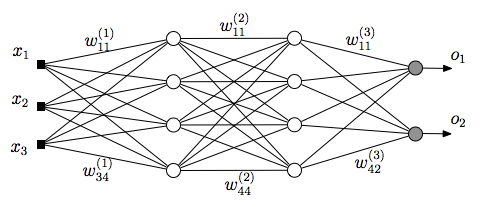
\includegraphics[scale=0.5]{img/MLP}
    \caption{Paveikslėlio pavyzdys}
    \label{img:mlp}
\end{figure}


\section{Eksperimentinio palyginimo rezultatai}
% tablesgenerator.com - converts calculators (e.g. excel) tables to LaTeX
\begin{table}[H]\footnotesize
  \centering
  \caption{Lentelės pavyzdys}
  {\begin{tabular}{|l|c|c|} \hline
    Algoritmas & $\bar{x}$ & $\sigma^{2}$ \\
    \hline
    Algoritmas A  & 1.6335    & 0.5584       \\
    Algoritmas B  & 1.7395    & 0.5647       \\
    \hline
  \end{tabular}}
  \label{tab:table example}
\end{table}

\end{document}
